%&latex
%
\providecommand{\main}{../..}
\documentclass[../../main.tex]{subfiles}

\begin{document}

\chapter{Ising Model}
\lesson{19}{22/04/20}

Statistical Mechanics, at its core, allows us to understand and quantify macroscopic phenomena starting from microscopic dynamics. In particular, it provides a window in how surprisingly \textit{complex} \textbf{emergent} behaviours arise from the interaction of many relatively \textit{simple}  components.

\medskip

One such example is given by \textbf{phase transitions},\marginpar{Phase transitions} i.e. abrupt changes of a system's properties when surpassing a well-defined threshold. For instance, water becomes ice when its temperature dips below $T=\SI{0}{\celsius}$, or steam when $T = \SI{100}{\celsius}$ is reached.

\medskip

Perhaps one of the simplest models describing a phase-transition is the \textbf{Ising Model}. At its origin, it was meant as an explanation of \textbf{ferromagnetism}. 

Certain \marginpar{Ferromagnetism and paramagnetism}materials possess no net magnetic moment above a certain temperature $T_c$ (the \textbf{Curie} temperature), and develop a temporary induced magnetization only in the presence of an external magnetic field (\textbf{paramagnetic} phase). However, when $T$ dips below $T_c$, they exhibit \textbf{spontaneous magnetization}, even in the absence of any external field, and behave like \textit{permanent magnets} (\textbf{ferromagnetic} phase).

\medskip

Classical Statistical Mechanics,\marginpar{Quantum nature of ferromagnetism} by itself, cannot explain this kind of behaviour. In fact, if we suppose that magnetization arises from \textit{tiny current loops}, its (canonical) thermal average is predicted to be always $0$, regardless of temperature\footnote{This is consequence of the Bohr-van Leeuwen theorem. See \cite{ferromagnets}}. 
This is because paramagnetism and ferromagnetism are inherently \textbf{quantum} phenomena, arising from the alignment of intrinsic magnetic dipoles of atoms, i.e. \textbf{spins}.

\medskip

In 1920, Wilhelm Lenz proposed a model of interacting spins on a lattice to his student Ernst Ising, who then found an analytic solution for the one-dimensional case in 1924. Underwhelmingly, the model did not exhibit any kind of phase transition - but it was still able to capture the attention of many researcher.

An analytic solution for the $d=2$ generalization was found by Lars Onsager in 1944, requiring a long and sophisticated mathematical derivation. In this case, however, the model was complex enough to capture a \textbf{phase transition} - a very important result for Statistical Mechanics. 

The Ising Model a lot of research and applications. %Add citation %"Exactly Solved Models in Statistical Mechanics" by R. J. Baxter
\marginpar{Applications} Nowadays, the Ising Model is relevant for simulating the behaviour of gases on a discretized grid (\textbf{lattice gases}), more complex \textbf{spin glasses}, and also the activity of \textbf{neural networks} (e.g. Hopfield networks). Also higher dimensional cases are of interest - for example the $d=4$ model is relevant for modelling \textit{spacetime} ($3$ dimensions for space plus $1$ for time). While no analytic solution for $d > 2$ is known, efficient numerical methods are available, and will be examined in a later chapter.

\section{Lattice gas}
The Ising Model can be introduced as a purely classical model when applied to the behaviour of gas particles in a discretized grid (lattice), completely bypassing the need to deal with quantum effects which are often difficult to interpret.

\medskip

Consider a system $\mathcal{S}$ of $N$ particles of mass $m$ enclosed in a volume $V$. Its state is completely specified by $3N$ positions and $3N$ momenta:
\begin{align*}
    \mathbb{Q} &= (q_{1x}, q_{1y}, q_{1z},\> \dots,\> q_{Nx}, q_{Ny}, q_{Nz}) = (\bm{q_1}, \dots, \bm{q_N})\in \mathbb{R}^{3N}\\
    \mathbb{P} &= (p_{1x}, p_{1y}, p_{1z},\>\dots, \> p_{Nx}, p_{Ny}, p_{Nz}) = (\bm{p_1}, \dots, \bm{p_N}) \in \mathbb{R}^{3N}
\end{align*}
Suppose that the particles interact through a potential $V_N(\mathbb{Q})$ depending only on the spatial coordinates. The Hamiltonian is then given by:
\begin{align}\label{eqn:hamiltonian-lattice}
    \mathcal{H}_{N}(\mathbb{Q}, \mathbb{P}) = \sum_{i=1}^N \frac{\norm{\bm{p_i}}^2}{2m} + V_N(\mathbb{Q})
\end{align}

The system is at equilibrium with a much larger environment, with which it exchanges both energy and particles. Denoting with $P$ the grand-canonical pressure, the grand-canonical partition function is given by:
\begin{align}\label{eqn:partition-lattice}
    e^{\beta P V} = \sum_{N=0}^{+\infty} \frac{1}{N!} \int_{\Gamma_N} \prod_{i=1}^N \frac{\dd[3]{\bm{q_i}} \dd[3]{\bm{p_i}}}{h^3} \exp(-\beta[ \mathcal{H}_N(\mathbb{Q}, \mathbb{P}) - \mu N])  
\end{align}
where $\mu$ is the system's chemical potential, representing the energy cost of adiabatically adding one particle to $\mathcal{S}$ such that the resulting $N+1$ system is still at equilibrium. Physically, the value of $\mu$ \textit{fixes} the average number of particles $\langle N \rangle$ in $\mathcal{S}$: if we \q{forcefully empty $\mathcal{S}$}, making $N=0$, particles will flow in $\mathcal{S}$ from the environment until the \q{cost} of adding a new particle reaches $\mu$, and then $N$ will only slightly oscillate.

\medskip

Since in (\ref{eqn:hamiltonian-lattice}) momenta and positions are independent, the integral over $\mathbb{P}$ in (\ref{eqn:partition-lattice}) is just a gaussian integral, resulting in:
\begin{align}\label{eqn:p-integ}
    \int_{\mathbb{R}^{3N}} \frac{\dd[3N]{\mathbb{P}}}{h^{3N}} \exp\left(-\beta\sum_{i=1}^N \frac{\norm{\bm{p_i}}^2}{2m} \right) = \left(\frac{2\pi m}{\beta h^2} \right)^{\frac{3N}{2}} \equiv \lambda^{-3N}
\end{align}
where:
\begin{align*}
    \lambda=\sqrt{\frac{\beta h^2}{2 \pi m}} \underset{\substack{\beta = 1/k_B T\\\hslash = h/2 \pi}}{=} \sqrt{\frac{2 \pi \hslash}{m k_B T}}
\end{align*}
is called the \textbf{thermal wavelength}\footnote{It is the average de Broglie wavelength of particles of an ideal gas at temperature $T$, i.e. of particles with energy of order $k_B T$.}, and has dimensions of a length (in fact $[\dd[3]{\bm{p}}/h^3] = 1/\si{\m^3}$). 

\medskip

Substituting (\ref{eqn:p-integ}) back in (\ref{eqn:partition-lattice}) leads to:
\begin{align}\nonumber
    e^{\beta P V} &= \sum_{N=0}^{+\infty} \frac{1}{N!} \int_{V^N} \dd[3N]{\mathbb{Q}} e^{-\beta V_N(\mathbb{Q})} \Bigg(\underbrace{\frac{e^{\beta \mu }}{\lambda^3}}_{z} \Bigg)^N =\\
    &= \sum_{N=0}^{+\infty}  \frac{z^N}{N!} \int_{V^N} \dd[3N]{\mathbb{Q}} e^{-\beta V_N(\mathbb{Q})}   \label{eqn:part-func}
\end{align}

We now \textbf{discretize} the\marginpar{1. Lattice discretization} system's volume $V$ in small cubic \textit{sites}, each with edges of size $a$ (fig. \ref{fig:lattices}). Space is thus divided in cells, each labelled by its $3$-dimensional integer indices $\bm{x_i} \in \mathbb{Z}^3$.

\medskip

More in general, we may consider a $d$-dimensional system, of $d$-volume\footnote{If $d=1$, then $V$ is a length, if $d=2$ it is an area, and if $d=3$ it is the usual volume. For higher dimensions it is a \textit{hyper}-volume.} $V$. Then, each cell $i$ will be labelled by $d$ indices: $\bm{x_i} \in \mathbb{Z}^d$. In fact, many physical systems can be modelled with $d\neq 3$ dimensions. For example, oxygen interacting with a graphite plane is intrinsically a $d=2$ system. 

\medskip

Also, cells may be of different shapes: it suffices that they are all equal and that they \textit{tessellate} the entire space. For instance, in $d=2$ we may subdivide a plane in triangles instead of squares, or with tetrahedra instead of cubes in $d=3$. In our case we will focus on the simplest choice, the cubic one. 

\medskip

Suppose now that $V_N(\mathbb{Q})$\marginpar{2. Pair-wise close-range potential} may be written as sum of two-body interactions:
\begin{align} \label{eqn:two-body-potential}
    V_N(\mathbb{Q}) = \sum_{i < j}^N v(q_{ij}) \qquad q_{ij} \equiv \norm{\bm{q_i}- \bm{q_j}}
\end{align}
where $v(q_{ij})$ is the potential of two particles $i$ and $j$ separated by a (relative) distance $q_{ij}$. If the gas is made of neutral particles, then $v(q)$ is a close-range attractive interaction, with the shape of a \textbf{Lennard-Jones potential} (fig. \ref{fig:lg-potential}). 

\begin{figure}[H]
    \centering
    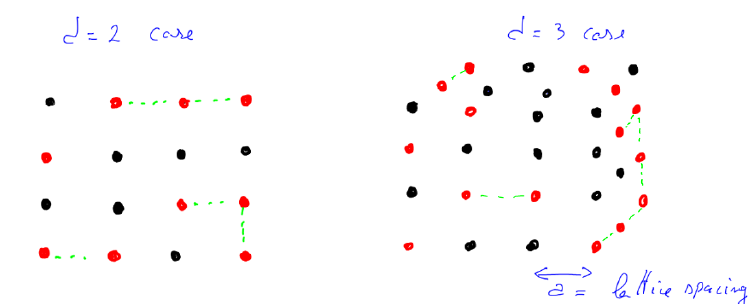
\includegraphics[width=0.6\textwidth]{\main/Images/image008.png}
    \caption{Examples of cubic lattices in $d=2$ and $d=3$.\label{fig:lattices}}
\end{figure}

\begin{figure}[H]
    \centering
    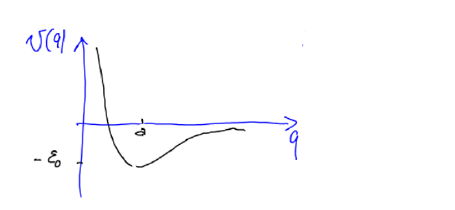
\includegraphics[width=0.6\textwidth]{\main/Images/image009.png}
    \caption{Shape of the Lennard-Jones potential. Two particles separated by a sufficiently small distance $q \sim a$ are weakly attracted to each other, and repelled if $q \to 0$ (as if they were \textit{hard spheres}). As $v(q)$ quickly vanishes for $q \to \infty$, particles that are too far from each other \textit{do not interact}. Physically, such $v(q)$ is due to interactions of the electronic clouds of neutral atoms. For $q$ too small, the (Pauli) repulsion of electrons dominates. Due to quantum fluctuations, the electronic clouds are not completely uniform: sometimes an electron \q{spends more time one one side}, producing a short-lived polarization. If $q \sim a$, one such \q{instantaneous dipole} may induce a temporary dipole in the other atom. It is this correlation between temporary polarizations that leads to a weak attractive force between the atoms (van der Waals force). \label{fig:lg-potential}}
\end{figure}

If we choose the lattice step length $a$ as the position of the minimum of $v(q)$, then on average at most one particle will occupy a given cell at any time - because two particles in the same site would be separated by $q < a$, for which $v(q)$ is strongly repulsive. Moreover, only particles in neighbouring cells are sufficiently close to interact with each other.

\medskip

So, in \textbf{approximation},\marginpar{3. Discretized potential} we consider a model in which cells can contain \textbf{at most one particle} at a time (at its centre), and interactions between non-neighbouring cells are neglected. Thus the distance $q$ between two particles must be a multiple of $a$, and the interaction potential is given by:
\begin{align*}
    v(q) = \begin{cases}
        +\infty & q = 0\\
        -\epsilon_0 & q=a\\
        0 & \text{otherwise}
    \end{cases}
\end{align*}

We then define the \textbf{occupancy} $n_i$ of cell $i$ as a binary variable:
\begin{align*}
    n_i = \begin{cases}
        1 & \text{Site $i$ contains a particle}\\
        0 & \text{Site $i$ is empty}
    \end{cases}
\end{align*} 
If we know all $\{n_i\}$, then the system (in this discretized approximation) is completely determined. Note that dealing with occupancies \textit{automatically} takes into account the indistinguishability of particles: $n_i = 1$ regardless if cell $i$ is occupied by particle $\#3$ or $\#42$.

\begin{appr}
    \textbf{Shortcomings of the lattice model}. In summary, the lattice model is a way to deal with the complex integration in \ref{eqn:part-func}, making the following approximations:
    \begin{enumerate}
        \item \textbf{Discretization}: space is divided in small cubic units, each containing \textbf{at most} one particle. 
        \item \textbf{Close-range pair-wise interaction}: the only possible interactions are between pairs of neighbouring cells.
    \end{enumerate}
    As a consequence of these approximation, there is a \textbf{maximum density} in the system, corresponding to the case when all cells are occupied - meaning that the system cannot be compressed over a certain threshold.
    
    Moreover, there is no way to understand if, in the densest case, particles are still moving from one cell to the other, \q{exchanging places} with each other, or if they just stay forever in their original site: in both cases, all the $n_i$ will be equal to $1$, and remain constant. In other words, there is no difference between the \textbf{liquid} phase and the \textbf{solid} one, meaning that the model \textbf{cannot appreciate the liquid-solid phase transition}, and so it is not very good for explaining the usual three phases of matter. However, it can describe accurately the liquid-vapour transition, and - more importantly - it leads to the Ising Model, which is very important in physical mechanics.

    \medskip

    There are of course more complex methods that relax the lattice approximation, dealing directly with the grand partition function in the continuum. In general they apply perturbation theory to the pair-wise potential, and through quite involved expansions (e.g. Virial expansion, or Mayer cluster expansion) they lead to equations of state capturing both the solid-liquid transition and the liquid-vapour transition. These are all well-known techniques (Mayer worked in the 1940s), with not much conceptual difficulty, apart of some very long and uninspiring computations. For more information, see \cite{huang}. 
\end{appr}

We can now write $V_N(\mathbb{Q})$ as function of the $\{n_i\}$. We consider two particles occupying neighbouring cells as being separated by a distance of $a$, and experiencing a potential $V(a) = -\epsilon_0$. Then the total potential experienced at cell $i$ is given by summing a contribution of $V(a)$ for each occupied neighbouring cell:
\begin{align*}
    V(\bm{x_i}) = - \epsilon_0\sum_{\langle j,i \rangle} n_j
\end{align*}
The notation $\langle j,i \rangle$ represents a sum over all cells $j$ that are the nearest neighbours of cell $i$. Then $\sum_{\langle j,i \rangle} n_j$ is exactly to the number of cells \textit{around} $i$ that are occupied. In particular, the total number $N$ of particles in the system is the number of occupied cells:
\begin{align}\label{eqn:num-particles1}
    N = \sum_x n_x
\end{align}

\medskip

Then, the total potential $V_N(\mathbb{Q})$ can be approximated as the sum of $V(\bm{x_i})$ terms over all cells $i$ that are occupied, leading to:
\begin{align}\label{eqn:total-pot1}
    V_N(\{\sigma_i\}) = - \epsilon_0 \sum_{\langle x,y \rangle} n_x n_y
\end{align}
Note that the product $n_x n_y$ is $1$ if and only if both cells are occupied.

So, in other words, $V_N$ is obtained by multiplying the average potential of an interaction ($-\epsilon_0$) by the number of such pairwise interactions, i.e. the number of pairs of neighbouring cells $\langle x,y\rangle$ that are both occupied.

\medskip

Note that not all sites are treated equally:\marginpar{Open and periodic boundary conditions} the ones at the \textbf{boundaries} of $V$ have a lower number of neighbours than the ones in the \textbf{bulk}. If we consider this asymmetry, letting cells at the margins interact only with their neighbours, the system is said to have \textbf{open boundaries}. Alternatively, boundaries may be removed by \q{connecting} sites at one margin with the ones from the opposite side (\textbf{periodic boundaries}). In this way, all cells have exactly the same number of neighbours, and can then be treated the same, achieving \textbf{translational invariance}.

\medskip

Periodic boundary conditions alter the system's \textbf{topology}.\marginpar{Periodic boundaries and topology} For example, in $d=1$, the \textit{open} case can be represented as a segment, while the \textit{periodic} one as a circle (fig. \ref{fig:1dperiodic}). In $d=2$, open boundaries result in a \textit{planar} topology, while periodic conditions produce a \textit{toroidal} surface (fig. \ref{fig:2dperiodic}).  

\begin{figure}[H]
    \centering
    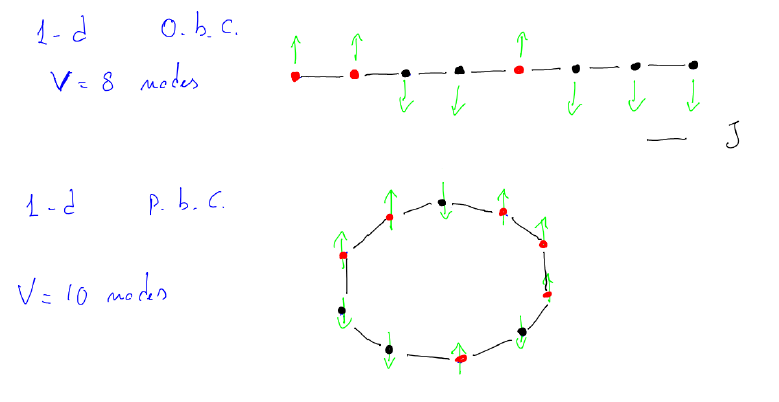
\includegraphics[width=0.8\textwidth]{\main/Images/image010.png}
    \caption{Ising model in $d=1$ with \textbf{open} boundaries (top), or \textbf{periodic} boundaries (bottom). Periodic conditions are obtained by \textit{deforming} the initial line to \q{attach} its two ends.\label{fig:1dperiodic}}
\end{figure}

\begin{figure}[H]
    \centering
    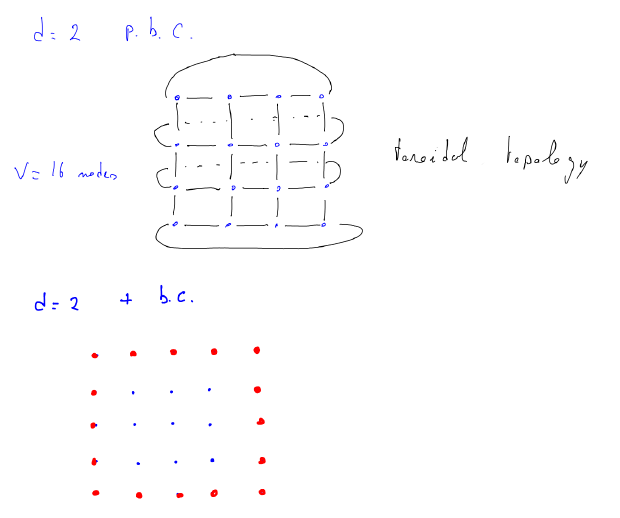
\includegraphics[width=0.8\textwidth]{\main/Images/image011.png}
    \caption{Ising model in $d=2$, with \textbf{periodic} boundaries (top) or \textbf{open} boundaries (bottom). Starting from a square, two opposite edges are attached together, forming a cylinder. Then the two circles at the boundaries are attached, deforming the cylinder into a torus.\label{fig:2dperiodic}}
\end{figure}

Boundaries may also be \textbf{fixed} to a particular \textit{state}: for example to be always empty or full of particles.

\medskip

It is now useful to \textit{shift} the occupancies $n_i$ so that they assume symmetrical values. So, we define a \q{spin-like} occupancy $\sigma_i$ as follows:
\begin{align}\label{eqn:spins}
    \sigma_i = \begin{cases}
        +1 & \text{Cell $i$ is occupied}\\
        -1 & \text{Cell $i$ is empty}
    \end{cases}
\end{align}
Clearly $\sigma_i = 2n_i - 1$, and so:
\begin{align*}
    n_i = \frac{1 + \sigma_i}{2} 
\end{align*}
And so we may rewrite (\ref{eqn:num-particles1}) and (\ref{eqn:total-pot1}) as follows:
\begin{align} \label{eqn:num-particles}
    N &= \sum_x \frac{1 + \sigma_x}{2}\\ 
    \label{eqn:total-pot}
    V_N(\{\sigma_i\}) &= - \epsilon_0 \sum_{\langle x,y \rangle} n_x n_y
\end{align}


We can then use (\ref{eqn:total-pot}) and (\ref{eqn:num-particles}) to approximate (\ref{eqn:part-func}) on the lattice:
\begin{align}\nonumber
    Z_{\mathrm{g.c.}} \equiv e^{\beta P V} &\underset{(\ref{eqn:part-func})}{=} \sum_{\{\bm{\sigma}\}} \exp(-\beta V_N(\bm{\sigma}) + N(\bm{\sigma}) \ln z) =\\
    &\underset{\substack{(\ref{eqn:total-pot})\\(\ref{eqn:num-particles})}}{=} \sum_{\{\bm{\sigma}\}} \exp \left(\beta \epsilon_0 \sum_{\langle x,y \rangle} \frac{1+\sigma_x}{2} \frac{1+\sigma_y}{2} + \ln z \sum_x \frac{1+\sigma_x}{2}   \right) \label{eqn:partition-discretized}
\end{align}
In fact the sum over all possible unique\footnote{Due to the division by $N!$, configurations where only $N$ cells are occupied are considered distinguishable only if the occupied cells are different. In other words, permuting the position of two particles is not counted.} configurations of $N$ particles over all values of $N$ is equivalent to the sum over all possible occupancies $\bm{\sigma} = \{\sigma_i\}$:
\begin{align*}
    \sum_{N=0}^{+\infty} \int_{V^N} \frac{\dd[d \cdot N]{\mathbb{Q}}}{N!} \xrightarrow[\text{discretization}]{} \sum_{\sigma_1 = \pm 1} \cdots \sum_{\sigma_\mathrm{last}  = \pm 1} = \sum_{\{\bm{\sigma}\}}
\end{align*}


\medskip

The choice of using spin-like variables (\ref{eqn:spins}) has lead to the appearance of constant terms, independent of the system's state, in (\ref{eqn:partition-discretized}), that we now extract. Consider the argument of the exponential, and expand the sums:
\begin{align}\label{eqn:expon}
    \frac{\beta \epsilon_0}{4} \left[\sum_{\langle x,y \rangle} 1 + \sum_{\langle x,y \rangle} (\sigma_x + \sigma_y) + \sum_{\langle x,y \rangle}\sigma_x \sigma_y\right] + \frac{\ln z}{2} \left(\sum_x 1 + \sum_x \sigma_x\right)
\end{align}
Summing ones over all cells is just the total number of cells in the lattice, each with volume $a^d$:
\begin{align*}
    \sum_x 1 = N_{\mathrm{cells}} = \frac{V}{a^d} 
\end{align*}
For simplicity, let's choose our units so that $a=1$, and thus:
\begin{align}\label{eqn:sum1}
    \sum_x 1 = V
\end{align}

\medskip

Similarly $\sum_{\langle x,y \rangle} 1$ counts the number of \textit{pairs} of neighbours. Graphically, if we represent cells as nodes in a graph, each connected to its neighbours by edges, then $\sum_{\langle x,y \rangle} 1$ is just the number of edges (fig. \ref{fig:1dperiodic}). Let's consider, for simplicity, a system with periodic boundary conditions - so that all cells have the same number $q$ of neighbours (this is also true for a system with open boundaries, in the limit of a lattice of infinite size). Then, the number of pairs (edges) will be:
\begin{align*}
    \sum_{\langle x,y \rangle} 1 = \text{N. of pairs} = \frac{N_{\mathrm{cells}} q}{2} = \frac{Vq}{2} 
\end{align*}
where the division by $2$ accounts for the fact that edges are \textit{undirected} - i.e. if $a$ is connected to $b$, then $b$ is connected to $a$ by the same edge. Without this division, we would be counting every edge \textit{twice}.  

\medskip

For a cubic lattice (with no boundaries), each cell has exactly $2$ neighbours in each \textit{direction}. So the total number of neighbours $q$ will be twice the number of dimensions $d$:
\begin{align}\label{eqn:sum2}
    \sum_{\langle x,y \rangle} 1 = \frac{2 V d}{2} = V d 
\end{align}

Finally, consider the second sum:
\begin{align*}
    \sum_{\langle x,y \rangle} \sigma_x + \sigma_y
\end{align*}
Practically, to compute it we may inspect each edge $(x,y)$, and sum the values $\sigma_x$ and $\sigma_y$ of the \textit{spins} at its extrema. When we are done, each value $\sigma_x$ at a node will have been considered exactly $q$ times - one for every neighbour of $x$:
\begin{align}\label{eqn:sum3}
    \sum_{\langle x,y \rangle} \sigma_x + \sigma_y = \sum_x \sigma_x \mathrm{dg}(x) 
\end{align}  
where $\mathrm{dg}(x)$ is the \textbf{degree} of node $x$, i.e. the number of connections (edges) involving cell $x$. In our case, $\mathrm{dg}(x) = q = 2d$:
\begin{align*}
    \sum_{\langle x,y \rangle} \sigma_x + \sigma_y = 2d \sum_x \sigma_x
\end{align*} 
This relation will allow to highlight the common factor $\sum_x \sigma_x$.

\medskip

Substituting (\ref{eqn:sum1}), (\ref{eqn:sum2}) and (\ref{eqn:sum3}) back in (\ref{eqn:expon}) leads to:
\begin{align}\nonumber
    &\phantom{=\>\>}\beta \frac{\epsilon_0}{4} \left[Vd + 2d \sum_x \sigma_x + \sum_{\langle x,y \rangle} \sigma_x \sigma_y\right]  + \frac{\ln z}{2} \left(V + \sum_x \sigma_x\right) =\\ \label{eqn:exponen2}
    &=\Bigg[\beta \underbrace{\frac{\epsilon_0}{4}}_{J} \sum_{\langle x,y \rangle} \sigma_x \sigma_y + \underbrace{\left[\frac{\beta \epsilon_0 d}{2}  + \frac{\ln z}{2} \right]}_{\beta b}  \sum_x \sigma_x \Bigg] + V\left( \beta \frac{\epsilon_0}{4} d +\frac{\ln z}{2} \right)
\end{align}
The term in the first set of square parentheses is the only one depending on $\bm{\sigma}$, and thus the one capturing the \textit{essence} of the Ising Model. The last one is just a scaling factor given by the current application (lattice gas).

\medskip

For simplicity, let's define:
\begin{align}\label{eqn:Jb}
    J \equiv \frac{\epsilon_0}{4}; \qquad \beta b \equiv \frac{\beta \epsilon_0 d}{2} + \frac{\ln z}{2}   
\end{align}
In this way we may collect a $\beta$ in (\ref{eqn:exponen2}):
\begin{align*}
    \beta \left[J \sum_{\langle x,y \rangle} \sigma_x \sigma_y + b \sum_x \sigma_x\right] + \beta V \left(J d + \frac{\ln z}{2 \beta} \right)
\end{align*}
Substituting back in (\ref{eqn:partition-discretized}):
\begin{align}\label{eqn:partition-3}
    Z_{\mathrm{g.c.}} \equiv e^{\beta PV} =\underbrace{ \left(\sum_{\{\bm{\sigma}\}} \exp\left[\beta \left(J \sum_{\langle x,y \rangle} \sigma_x \sigma_y + b \sum_x \sigma_x\right)\right] \right)}_{Z} \exp\left(\beta V \left[Jd + \frac{\ln z}{2 \beta} \right]\right)
\end{align}
We define the Ising Model partition function $Z$ to contain the only relevant factor:
\begin{align} \label{eqn:Z-ising}
    Z_{\mathrm{Ising}} \equiv \sum_{\{\bm{\sigma}\}} \exp\left[\beta \left(J \sum_{\langle x,y \rangle} \sigma_x \sigma_y + b \sum_x \sigma_x\right)\right] \equiv e^{-\beta V f(T,b)}
\end{align}
where $f(T,b)$ (defined by the above relation) is the model's \textbf{free energy density}. Then, taking the logarithm of both terms in (\ref{eqn:partition-3}):
\begin{align}\label{eqn:calc4}
    \cancel{\beta }P \cancel{V} \underset{(\ref{eqn:Z-ising})}{=}  -\cancel{\beta V} f(T,b) +\cancel{ \beta V} J d + \cancel{\beta V} \frac{\ln z}{2 \beta} 
\end{align}
Rearranging the definition of $b$ (\ref{eqn:Jb}):
\begin{align*}
    b = \frac{\epsilon_0 d}{2} + \frac{\ln z}{2 \beta} \Rightarrow \frac{\ln z}{2 \beta} = b - \frac{\epsilon_0 d}{2}    
\end{align*}
and substituting in (\ref{eqn:calc4}) we get the grand-canonical pressure of the lattice gas:
\begin{align}\nonumber
    P_{\mathrm{g.c.}} &= -f(T,b) + \frac{\epsilon_0}{4} d + b - \frac{\epsilon_0 d}{2} = -f(T,b) -\frac{\epsilon_0}{4} d + b =\\
    &= -f(T,b) +b - Jd   \label{eqn:Pgc}
\end{align}

The physical interpretation of $J$ and $b$ depends on which application we are considering. In the lattice gas, $J$ is clearly proportional to the strength of interaction between gas molecules occupying neighbouring cells, while $b$ depends on the chemical potential $\mu$ (through $z$), the temperature and the system's dimensionality. 

A clearer meaning for $b$ is found when the Ising Model is applied to ferromagnetism. In this case, the $\{\sigma_i\}$ represent the direction (up or down) of the particle's \textit{spins}, i.e. their \textit{intrinsic} magnetic momenta (of pure quantum origin). Then $b \sum_x \sigma_x$ measures the correlation between the \textit{spin directions} and $b$. In particular, configurations for which the majority of $\sigma_i$ have the same sign of $b$ (i.e. are \q{parallel} to $b$) have a higher probability (as each term in the sum over states in $Z$ is the probability associated with a particular configuration $\bm{\sigma}$). So, $b$ can be interpreted as an \textbf{external magnetic field}, pushing each particle to align its spin to it.

On the other hand, for a quantum system (such as a ferromagnet), $J$ is called the \textbf{exchange energy}, and measures the overlap of electronic clouds of neighbouring atoms. 

\medskip

From (\ref{eqn:Z-ising}) we can extract the Hamiltonian for the Ising Model:
\begin{align}\label{eqn:H-ising}
    Z_{\mathrm{Ising}} \equiv \sum_{\{\bm{\sigma}\}} e^{-\beta \mathcal{H}(\bm{\sigma})} \Rightarrow \mathcal{H}(\bm{\sigma}) = -J \sum_{\langle x,y \rangle} \sigma_x \sigma_y - b \sum_x \sigma_x
\end{align}

$\beta \mathcal{H}(\bm{\sigma})$ is called the \textbf{reduced Hamiltonian}:
\begin{align*}
    \beta \mathcal{H}(\bm{\sigma}) &= -\underbrace{\beta J}_{K} \sum_{\langle x,y \rangle} \sigma_x \sigma_y -\underbrace{\beta b}_{h} \sum_x \sigma_x \\
    &= -K \sum_{\langle x,y \rangle} \sigma_x \sigma_y - h \sum_x \sigma_x
\end{align*}  

%Approximation of quantum system, Pauli matrices, paragraph by Sethna (add green box)

Intuitively, $\mathcal{H}(\bm{\sigma})$ is the sum of two interactions:
\begin{itemize}
    \item \textbf{Spin-spin interactions}: $-J \sum_{\langle x,y \rangle} \sigma_x \sigma_y$. If $J > 0$, the term is minimized if $\sigma_x \sigma_y > 0$, i.e. if neighbouring spins are all \textit{parallel} to each other (\textbf{ferromagnetic order}). If $J < 0$, spins tend instead to be \textit{anti-parallel} to each other (\textbf{anti-ferromagnetic order}), as can be seen in fig. \ref{fig:orders}. 
    \item \textbf{Spin-field interaction}: $-b \sum_x \sigma_x$, which is minimized if spins are aligned (parallel) to the magnetic field $b$ (when applying the model to a ferromagnet).  
\end{itemize}
In particular, if $h = 0$ (and so $b=0$), then there is no \q{preferred direction} for the alignment of spins. This results in two equivalent \textit{ground states}, as $H(\bm{\sigma}) = H(-\bm{\sigma})$. For instance, if $J > 0$, the two possibilities are all $\sigma_i = +1$ (up), or all $\sigma_i = -1$ (down).

\begin{figure}[H]
    \centering
    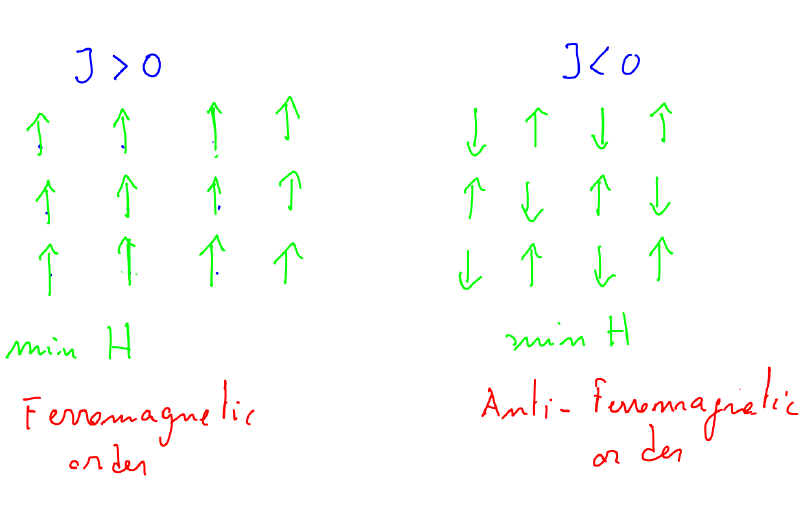
\includegraphics[width=0.7\textwidth]{\main/image013.png} 
    \caption{The spin-spin interaction energy when all neighbouring spins are ordered in a (anti)parallel way, depending on the sign of $J$.\label{fig:orders}}
\end{figure}

\section{Ising Partition Function}
Our next goal is to compute explicitly the Ising partition function (\ref{eqn:Z-ising}):
\begin{align}\label{eqn:Z-Is}
    Z(K,h) = \sum_{\{\bm{\sigma}\}} \exp\left(K \sum_{\langle x,y \rangle} \sigma_x \sigma_y + h \sum_x \sigma_x\right) = e^{-\beta V f(K,h)} \qquad \substack{K = \beta J\\h = \beta b}
\end{align}
Note that the sum is over $2^{N_{\mathrm{cells}}} = 2^V$ (as the lattice step $a$ is set to $1$) possible states (spin configurations).

\medskip

We define the\marginpar{Magnetization}\index{Magnetization} \textbf{magnetization} $m$ as the average \textit{alignment} of spins:
\begin{align} \nonumber
    m &\equiv \frac{1}{V} \langle \sum_x \sigma_x \rangle =  \frac{1}{V} \frac{1}{Z} \sum_{\{\bm{\sigma}\}} \exp\left(K \sum_{\langle x,y \rangle} \sigma_x \sigma_y + h \sum_x \sigma_x\right) \sum_x \sigma_x =\\
    &= \frac{1}{V} \pdv{h} \ln Z(K, h) \underset{(\ref{eqn:Z-Is})}{=}  - \beta \pdv{h} f(K,h)  \label{eqn:magnetization}
\end{align}  

The average number of particles\marginpar{Average number of particles $\langle N \rangle$} $\langle N \rangle$ in a grand-canonical ensemble is given by:
\begin{align} 
    \langle N \rangle_{\mathrm{g.c.}} = \frac{1}{\beta} \pdv{\mu} \ln Z_{\mathrm{g.c.}} = \frac{1}{\beta} \pdv{\textcolor{Red}{z}}{\mu} \pdv{\textcolor{Red}{z}} \ln Z_{\mathrm{g.c.}}
\end{align}
with:
\begin{align*}
    \pdv{z}{\mu} = \pdv{\mu} \frac{e^{\beta \mu}}{\lambda^3} = \beta \underbrace{\frac{e^{\beta \mu}}{\lambda^3}}_{z} = \beta z 
\end{align*}
and so:
\begin{align}\label{eqn:avgN}
    \langle N \rangle_{\mathrm{g.c.}} = \frac{1}{\cancel{\beta}} \cancel{\beta} z \pdv{z} \ln Z_{\mathrm{g.c.}} = z \pdv{z} \ln Z_{\mathrm{g.c.}}
\end{align}
Let $v$ be the average volume per particle\marginpar{Particle density}, i.e. $\langle N \rangle/V$. Then the average \textbf{density} of particles is $v^{-1}$:
\begin{align}\nonumber
    v^{-1} &\equiv \frac{\langle N \rangle}{V} \underset{(\ref{eqn:avgN})}{=}  \frac{z}{V}  \pdv{z} \ln Z_{\mathrm{g.c.}} \underset{(\ref{eqn:partition-3})}{=} \frac{z}{V} \pdv{z} \beta P V =\\ \nonumber
    &\underset{\mathclap{(\ref{eqn:Pgc})}}{=}\>  \frac{z}{V} \pdv{z} \left[-\beta V f(T,b(z)) +\beta V b(z)  - \beta V J d\right] =\\
    &\underset{\mathclap{(\ref{eqn:Z-Is})}}{=} \> \frac{z}{V} \pdv{z} [\hlc{ForestGreen}{\ln Z_{\mathrm{Ising}}} + \hlc{SkyBlue}{\beta V b}] \label{eqn:v-1}
\end{align}
as the third term does not depend on $z$. It is useful to change variables from $z \to \ln z$, as $b$ is a function of $\ln z$:
\begin{align*}
    z\pdv{z} = z \pdv{(\textcolor{Red}{\ln z})}{z} \pdv{\textcolor{Red}{(\ln z)}} = \cancel{z} \frac{1}{\cancel{z}} \pdv{(\ln z)} = \pdv{(\ln z)} 
\end{align*}
So that:
\begin{align}\label{eqn:dv1}
    \hlc{SkyBlue}{\frac{z}{\cancel{V}} \pdv{z} \beta \cancel{V} b} = \beta  \pdv{b}{(\ln z)} \underset{(\ref{eqn:Jb})}{=}  \cancel{\beta } \frac{1}{2\cancel{ \beta }} = \frac{1}{2} 
\end{align}
With another change of variable $z \to h$ we can rewrite $z \partial_z \ln Z_{\mathrm{Ising}}$ as a function of the magnetization $m$:
\begin{align}\label{eqn:dv2}
    \hlc{ForestGreen}{\frac{z}{V} \pdv{z} \ln Z_{\mathrm{Ising} }} =  \pdv{\textcolor{Red}{h}}{(\ln z)} \underbrace{\frac{1}{V}\pdv{\textcolor{Red}{h}} \ln Z_{\mathrm{Ising}}}_{m} = \left(\pdv{(\ln z)}{(h)}\right)^{-1} m \underset{(a)}{=}  \frac{m}{2} 
\end{align}
where the derivative in (a) can be computed by isolating $\ln z$ in the definition of $b$ (\ref{eqn:Jb}):
\begin{align*}
    b = \frac{\epsilon_0 d}{2} + \frac{\ln z}{2 \beta} \Rightarrow 2 \beta b = \underbrace{\epsilon_0 }_{4J}d \beta + \ln z \Rightarrow \ln z = 2\beta(b - 2 J d) = 2(h- 2 K d) \Rightarrow \pdv{(\ln z)}{h} = 2
\end{align*}

Substituting (\ref{eqn:dv1})\marginpar{Particle density and magnetization} and (\ref{eqn:dv2}) back in (\ref{eqn:v-1}) leads to:
\begin{align}\label{eqn:v-density}
    v^{-1} = \frac{m}{2} + \frac{1}{2} = \frac{m+1}{2}   
\end{align}
So a higher $m$ corresponds (in the lattice gas model) to a higher particle density. Intuitively, a high $m$ means that, \textit{on average}, cells are more occupied - meaning that particles will be, in general, closer together. Note that $m \in [-1,+1]$ (which happens, respectively, when all spins point \textit{up} or \textit{down}, i.e. if all cells are occupied or empty), and so $v^{-1} \in [0, 1]$ as expected. 

\medskip

Assuming periodic boundary conditions,\marginpar{Consequences of translational invariance} the system is \textbf{translational invariant}: there is no \q{preferred} position in the lattice - all cells are exactly equal to each other. This means that $\langle \sigma_x \rangle \equiv \bar{\sigma}$ must be independent of $x$, and so it is equal to the magnetization $m$:
\begin{align*}
    m = \frac{1}{V} \langle \sum_x \sigma_x \rangle =  \frac{1}{V} \sum_x \langle \sigma_x \rangle = \frac{1}{\cancel{V}} \cancel{V} \bar{\sigma} = \bar{\sigma} = \langle \sigma_x \rangle
\end{align*}
On the other hand, the $2$-point correlation function $\langle \sigma_x \sigma_y \rangle$ must depend only on the distance $\norm{\bm{r}_x - \bm{r}_y}$ between the two cells, because of translational invariance. 

\medskip

Note that for any finite $V$, the sum in (\ref{eqn:Z-Is}) is a sum over a finite number $2^V$ of states. As each term is an analytic function, $Z$ is also an analytic function, and so it is $\ln Z = - \beta V f(K,h)$, and in particular the free energy $f(K,h)$. However, we expect phase-transitions to correspond to points at which the free energy is non-analytic - which would explain the \textit{sudden} changes in the system's properties that are experimentally observed during such a transition. %Motivate 

So, in any finite lattice we won't be able to see any phase-transition. Conversely, to observe a phase-transition, an \textbf{infinite lattice} is required, which is obtained when $V \to \infty$, i.e. in the \textbf{thermodynamic limit}. 

\begin{example}[Non-interacting spins]
    Let's examine the simplest possible case in the Ising Model, occurring when $J=0$ (or, equivalently, $K=0$). The Hamiltonian becomes:
    \begin{align}\label{eqn:free-H}
        \mathcal{H}(\bm{\sigma}) = -h \sum_x \sigma_x
    \end{align}
    meaning that spins (or cells) are completely independent from each other (\textbf{decoupled}). In fact, the partition function factorizes:
    \begin{align*}
        Z= \sum_{\{\bm{\sigma}\}} \exp({h \sum_x \sigma_x}) = \sum_{\sigma_1 = \pm 1} e^{h \sigma_1} \cdots \sum_{\sigma_V = \pm 1}e^{h \sigma_V}
    \end{align*}
    Noting that:
    \begin{align*}
        \sum_{\sigma_i = \pm 1} e^{h \sigma_i} = \textcolor{Red}{2} \frac{e^{h} + e^{-h}}{\textcolor{Red}{2}} = 2 \cosh h
    \end{align*}
    the partition function becomes:
    \begin{align} \label{eqn:free-Z}
        Z = (2 \cosh h)^V
    \end{align}
    Then the \textbf{free energy} $f$ is:
    \begin{align}\label{eqn:free-f}
        Z = e^{- \beta V f(h)} \Rightarrow f(h) = - \frac{\ln Z}{\beta V} \underset{(\ref{eqn:free-Z})}{=}  -\frac{\ln(2 \cosh h)}{\beta}
    \end{align}
    The \textbf{magnetization}:
    \begin{align}\label{eqn:mh}
        m(h) \underset{(\ref{eqn:magnetization})}{=}  -\beta \pdv{h}f(h) = \pdv{h} \ln(\cosh h) = \frac{\sinh h}{\cosh h} = \frac{e^h - e^{-h}}{e^{h} + e^{-h}} = \tanh h  
    \end{align}
    A plot of $m(h)$ can be seen in fig. \ref{fig:free-spin-m}. 

    Inverting (\ref{eqn:mh}) allows to express $h$ as a function of $m$:
    \begin{align*}
        h = \beta b = \tanh^{-1} m
    \end{align*}
    This can be solved by letting $t = e^h$, and so:
    \begin{align*}
        m = \tanh h = \frac{t + 1/t}{t-1/t} = \dfrac{\frac{t^2-1}{\bcancel{t}}}{\frac{t^2+1}{\bcancel{t}}} \Rightarrow m(t^2 +1) = t^2 - 1 \\ \Rightarrow t^2 (m-1) = -(m+1) \Rightarrow t= \pm \sqrt{\frac{1+m}{1-m} } \span
    \end{align*}
    As $t = e^h > 0$, only the positive solution is acceptable, leading to:
    \begin{align*}
        e^h = \sqrt{\frac{1+m}{1-h}} \Rightarrow h = \ln \sqrt{\frac{1+m}{1-h} } = \frac{1}{2} \ln \frac{1+m}{1-m}  
    \end{align*}
    Substituting back:
    \begin{align}\label{eqn:hm}
        h = \beta b = \tanh^{-1} m = \frac{1}{2} \ln \frac{1+m}{1-m} \qquad -1 < m < +1 
    \end{align}
    We can also express the free energy (\ref{eqn:free-f}) as function of $m$. First note that:
    \begin{align}\nonumber
        \ln \cosh h &= \frac{1}{\textcolor{Red}{2}} \ln (\cosh h)^{\textcolor{Red}{2}} = \frac{1}{2} \ln \frac{\textcolor{Magenta}{\cosh^2 h}}{\underbrace{\textcolor{Blue}{\cosh^2 h - \sinh^2 h}}_{1}} = \\ \nonumber
        &= \textcolor{Red}{-}\frac{1}{2} \ln \frac{\textcolor{Blue}{\cosh^2 h - \sinh^2 h}}{\textcolor{Magenta}{\cosh^2 h}} =- \frac{1}{2} \ln (1 - \tanh^2 h) =\\ \label{eqn:logcosh}
        &\underset{(\ref{eqn:hm})}{=} - \frac{1}{2} \ln (1 - m^2)  
    \end{align}
    and so:
    \begin{align}\nonumber
        f \underset{\mathclap{(\ref{eqn:free-f})}}{=}\> -\frac{\ln (2 \cosh h)}{\beta} \Rightarrow \beta f &=  -\ln(\cosh h) - \ln 2 = \\
        &\underset{\mathclap{(\ref{eqn:logcosh})}}{=}\> \frac{1}{2} \ln (1-m^2) - \frac{1}{\textcolor{Red}{2}} \ln 2^{\textcolor{Red}{2}} = \frac{1}{2} \ln \frac{1-m^2(h)}{4}  \label{eqn:f-h}
    \end{align}
    Note that the free energy is an \textbf{even} function of the magnetization, whereas $m$ is an \textbf{odd} function of $h$. 

    \medskip

    Finally, from (\ref{eqn:mh}) note that the derivative of $f$ with respect to $b$ is $-m$:
    \begin{align*}
        \pdv{f}{b} = \pdv{f}{h} {\pdv{h}{b}} \underset{\substack{h = \beta b\\(\ref{eqn:mh})}}{=} -\frac{m}{\cancel{\beta}} \cancel{\beta} = -m
    \end{align*}

    So, the \textcolor{Magenta}{(non-standard)} \textbf{Legendre transform} of $f(b)$ with respect to $b$ is $\gamma(m)$ defined by the following relation:
    \begin{align}\label{eqn:leg-tran-f}
        \textcolor{Magenta}{-} \gamma(m) + f(b(m)) = {\pdv{f}{b}}  \cdot b(m) = -mb(m) \Rightarrow \gamma(m) = f+ bm
    \end{align} 
    $b(m)$ is obtained rearranging (\ref{eqn:hm}):
    \begin{align}\label{eqn:sub1}
        \frac{h}{\beta} = b = \frac{1}{2\beta} \ln \frac{1+m}{1-m}   
    \end{align}
    Then substituting (\ref{eqn:f-h}) and (\ref{eqn:sub1}) in (\ref{eqn:leg-tran-f}) leads to:
    \begin{align*}
        \gamma(m) &= \frac{1}{2 \beta} \ln \frac{1-m^2}{4} + \frac{m}{2\beta}\ln \frac{1+m}{1-m} =\\
        &=\frac{1}{2\beta} \left[\ln \frac{1-m}{2} \frac{1+m}{2} + m\left(\ln \frac{1+m}{\textcolor{Red}{2}} +\textcolor{Red}{\cancel{\ln 2}} - \ln\frac{1-m}{\textcolor{Blue}{2}} -\textcolor{Blue}{\cancel{\ln 2}}   \right)    \right] =\\
        &= \frac{1}{2\beta} \left[\ln \frac{1-m}{2} + \ln \frac{1+m}{2} + m\left(\ln \frac{1+m}{2} - \ln \frac{1-m}{2}  \right)\right] =\\
        &= \frac{1}{2\beta} \left[(1+m)\ln\frac{1+m}{2} +(1-m) \ln \frac{1-m}{2}  \right] =\\
        &= \left[\frac{1-m}{2} \ln \frac{1-m}{2} +\frac{1+m}{2}\ln \frac{1+m}{2}    \right] \beta^{-1}
    \end{align*} 
    Note that, due to the properties of the Legendre transform, we have:
    \begin{align*}
        \pdv{\gamma(m)}{m} = b
    \end{align*}

    %Check from here------ (Last 10 minutes)
    Then, the \textbf{entropy density} is obtained by differentiating $f$ (or equivalently its Legendre transform $\gamma$, as $T$ is not involved in the transformation):
    \begin{align}\label{eqn:s-density}
        s = -\pdv{f}{T} = -\pdv{\gamma}{T} = -k_B \left[\frac{1-m}{2} \ln \frac{1-m}{2} + \frac{1+m}{2} \ln \frac{1+m}{2} \right]
    \end{align} 

    This can be derived also from the definition of the Shannon Entropy. Recall that the probability of a certain spin configuration $\bm{\sigma}$ is:
    \begin{align*}
        \rho(\bm{\sigma}) = \frac{1}{Z} e^{- \beta \mathcal{H}(\bm{\sigma})} 
    \end{align*}
    As spins are decoupled, $\rho(\bm{\sigma})$ factorizes: 
    \begin{align}\label{eqn:rho1}
        \rho(\bm{\sigma}) \underset{\substack{(\ref{eqn:free-H})\\(\ref{eqn:free-Z})}}{=}  \prod_x \frac{e^{h \sigma_x}}{2 \cosh h}  \equiv \prod_x \rho_1(\sigma_x) \qquad \rho_1(\sigma_x) \equiv \frac{e^{h \sigma_x}}{2 \cosh h} 
    \end{align}

    Any generic function $g(\sigma)$ of a binary variable $\sigma \in \{\pm 1\}$ can be written as:
    \begin{align*}
        g(\sigma) = \frac{g(+1) + g(-1)}{2} + \sigma \frac{g(+1) - g(-1)}{2}  
    \end{align*}
    In fact:
    \begin{align*}
        g(+1) &= \frac{g(+1) + \cancel{g(-1)}}{2} +\frac{g(+1) - \cancel{g(-1)}}{2} = g(+1)\\
        g(-1) &= \frac{\cancel{g(+1)} + g(-1)}{2} - \frac{\cancel{g(+1)} - g(-1)}{2} = g(-1)
    \end{align*}

    In particular, if $g(\sigma) = \exp(h \sigma)$:
    \begin{align}\label{eqn:ehsigma}
        e^{h \sigma} = \frac{e^h + e^{-h}}{2} + \sigma \frac{e^h - e^{-h}}{2} = \cosh h + \sigma \sinh h  
    \end{align}
    And so:
    \begin{align}\label{eqn:rho1-m}
        \rho_1(\sigma) \underset{(\ref{eqn:rho1})}{=}  \frac{e^{h \sigma}}{2 \cosh h} \underset{(\ref{eqn:ehsigma})}{=} \frac{\cosh h + \sigma \sinh h}{2 \cosh h} = \frac{1+\sigma \tanh h}{2} \underset{(\ref{eqn:mh})}{=}  \frac{1 + \sigma m}{2} 
    \end{align}
    The $\rho_1$ so defined is already normalized:
    \begin{align} \label{eqn:normalizrho1}
        \sum_{\sigma = \pm 1} \rho_1(\sigma) = \frac{1+\cancel{m}}{2} + \frac{1-\cancel{m}}{2} =   1
    \end{align}
    We are now ready to compute the \textbf{information entropy}:
    \begin{align}\nonumber
        S_I[\rho] &= -k_B \sum_{\{\bm{\sigma}\}} \rho(\bm{\sigma}) \ln \rho(\bm{\sigma}) \underset{(\ref{eqn:rho1})}{=}  -k_B \hlc{Yellow}{\sum_{\{\bm{\sigma}\}}} \left(\prod_{x=1}^V \rho_1(\sigma_x)\right) \ln \left(\prod_{y=1}^V \rho_1(\sigma_y)\right) =\\ \nonumber
        &=-k_B \hlc{Yellow}{\sum_{\sigma_1 = \pm 1} \cdots \sum_{\sigma_V = \pm 1}} \hlc{SkyBlue}{\prod_{x=1}^V \rho_1(\sigma_x)} \textcolor{Blue}{\sum_{y=1}^V} \ln \rho_1(\sigma_y) =\\ \nonumber
        &\underset{(a)}{=}  -k_B \textcolor{Blue}{\sum_{y=1}^V} \sum_{\sigma_1 = \pm 1} \cdots \sum_{\sigma_V = \pm 1} \hlc{SkyBlue}{\Big(\prod_{x \neq y} \rho_1(\sigma_x)\Big) \rho_1(\sigma_y)} \ln \rho_1 (\sigma_y) =\\\nonumber
        &\underset{(b)}{=}  -k_B \sum_{y=1}^{V} \sum_{\sigma_y = \pm 1} \rho_1(\sigma_y) \ln \rho_1(\sigma_y) \prod_{x \neq y} \underbrace{\sum_{\sigma_{x} = \pm 1} \rho_1(\sigma_x)}_{1} =\\
        &\underset{(c)}{=}  -k_B \sum_{y=1}^V \sum_{\sigma_y = \pm 1} \rho_1(\sigma_y) \ln \rho_1(\sigma_y) = -k_B V \sum_{\sigma_y = \pm 1} \rho_1(\sigma_y) \ln \rho_1(\sigma_y) \label{eqn:lstep}
    \end{align}
    In (a) we exchange the sum over cells $y$ with the one over states $\bm{\sigma}$. Then, we split the product over $x$ (highlighted in blue) in two factors: one with $x \neq y$, and the other with $x=y$. Then, in (b) we exchange the order of the sums over cell states, bringing the one over $\sigma_y$ first, and factoring out everything that depends only on $\sigma_y$. The remaining term is a product of $\rho_1$, and thanks to the spin-independence we can bring all the other sum over states inside it, and then apply normalization (\ref{eqn:normalizrho1}) to reach the result in (c). Due to translational invariance, the inner sum evaluates to a constant, and so $\sum_{y=1}^V$ amounts merely to multiplying by the number of cells $V$.

    \medskip

    Finally, substituting (\ref{eqn:rho1-m}) in the last step (\ref{eqn:lstep}) and dividing by $V$ leads back to (\ref{eqn:s-density}):
    \begin{align}\label{eqn:lstepb}
        s = \frac{S_I[\rho]}{V} = -k_B\left[\frac{1+m}{2} \ln \frac{1+m}{2} + \frac{1-m}{2} \ln \frac{1-m}{2} \right] 
    \end{align}

    The grand-canonical pressure is given by:
    \begin{align*}
        P &\underset{(\ref{eqn:Pgc})}{=}  [-f(T,b) + b - Jd]\Big|_{J=0} \underset{\substack{(\ref{eqn:f-h})\\(\ref{eqn:sub1})}}{=} -\frac{1}{2\beta} \ln \frac{1-m^2}{4} + \frac{1}{2\beta} \ln \frac{1+m}{1-m} = \\
        &=\frac{1}{2\beta} \left[-\ln \frac{1-m}{2} -\cancel{ \ln \frac{1+m}{2}} + \cancel{\ln \frac{1+m}{2} }- \ln \frac{1-m}{2}    \right] = -\beta^{-1} \ln \frac{1-m}{2} =\\
        &=-\beta^{-1} \ln \frac{\textcolor{Red}{2} - \textcolor{Red}{1}-m}{2} = -\beta^{-1} \ln\left(1-\frac{m+1}{2} \right) \underset{(\ref{eqn:v-density})}{=} -\beta^{-1} \ln(1- v^{-1}) =\\
        &= - \beta^{-1} \ln \left(1-\frac{\langle N \rangle}{V} \right) \xrightarrow[v^{-1} \to 0]{} -\beta^{-1} \left(-\frac{\langle N \rangle}{V}\right) = k_B T \frac{\langle N \rangle}{V} 
    \end{align*}
    So, in the limit of \textit{low density} $v^{-1} \to 0$, i.e. of a rarefied gas, we get the equation of state for an ideal gas in the grand-canonical ensemble.

    \medskip

    However, if we consider the full equation, we note a singularity for $v^{-1} \to 1$ (densest case, where all cells are filled), corresponding to the \textit{liquid phase}. A plot of $P(v)$ is shown in fig. \ref{fig:pressure}, and compared with the one of a real gas. In particular, no \textit{phase-transition} is captured by such \textit{free} Ising Model: as we will see, spin-spin interactions are fundamental. However, even with $J=0$, the model is able to describe two phases: that of a rarefied gas and of a liquid.
\end{example}

\begin{figure}[H]
    \centering
    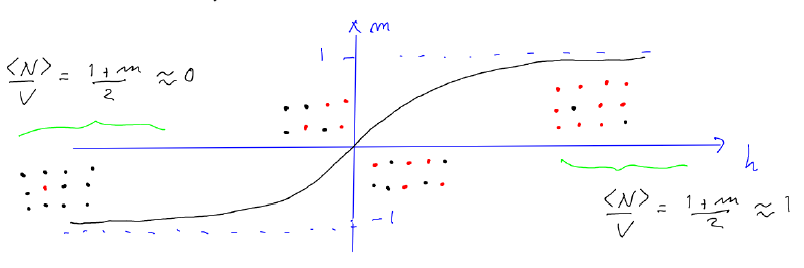
\includegraphics[width=0.8\textwidth]{\main/Images/image014.png}
    \caption{Magnetization $m$ as function of $h = \beta b$ for the Ising Model with decoupled spins ($J=0$). For $h \to \pm \infty$, $m = \tanh h \to \pm 1$. For the negative magnetization, the lattice is almost \q{empty}, while for $m \to +1$ it is almost full.
    \label{fig:free-spin-m}} 
\end{figure} 


\begin{figure}[H]
    \centering
    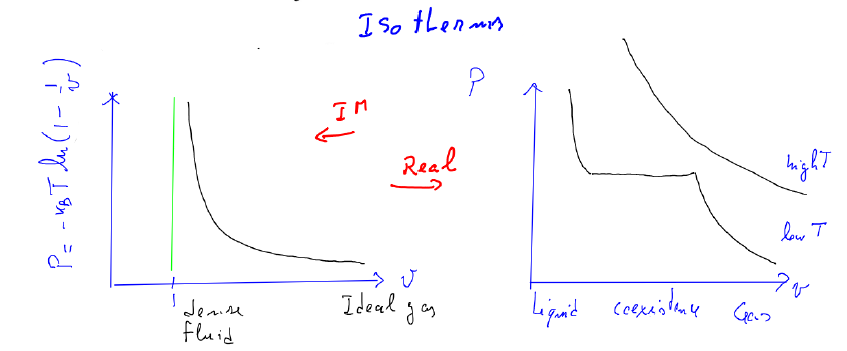
\includegraphics[width=0.8\textwidth]{\main/Images/image015.png}
    \caption{Isothermal curves $P(v)$ for the lattice gas (left) and a real gas (right), where $v$ is the average volume per particle (the reciprocal of the density $v^{-1}$). In the Ising Model pressure \textit{diverges} when density approaches its maximum $v^{-1} \to 1$. However, in the real case there is a range of temperatures at which, for a range of values of $v$, the liquid and gas phases are coexisting (which is where the phase transition is happening). So the model is able to capture \textit{some} of the behaviour (the dilute \q{ideal gas} state and the \textit{liquid} phase), but not all. 
    \label{fig:pressure}} 
\end{figure} 

\begin{exo}[2-point correlation]
    Show that:
    \begin{align*}
        \langle \sigma_x \sigma_y \rangle = (\tanh h)^2 = \langle \sigma_x \rangle \langle \sigma_y \rangle
    \end{align*} %Is this in the free Ising model?
\end{exo}



\end{document}
